% ~~~~~~~~~~~~~~~~~~~~~~~~~~~~~~~~~~~~~~~~~~~~~~~~~~~~~~~~~~~~~~~~~~~~~~~~~~~~~
%                                 RESULTS
% ~~~~~~~~~~~~~~~~~~~~~~~~~~~~~~~~~~~~~~~~~~~~~~~~~~~~~~~~~~~~~~~~~~~~~~~~~~~~~
\chapter{Results}\label{chap:5}
  \lhead{Chapter 5. \emph{Results}}

Although I have tested multiple variations of the algorithm, I could not
find the right setting for network to learn.

Maybe, input for the network could
be better.

% The only pattern
% {\lstinline{QLNNPlayer}} could learn was to move straight down until hit
% the first wall.

\graphicspath{{plots/}}

\begin{wrapfigure}{L}{0.5\textwidth}
  \vspace*{-0.20cm}
  \centering
  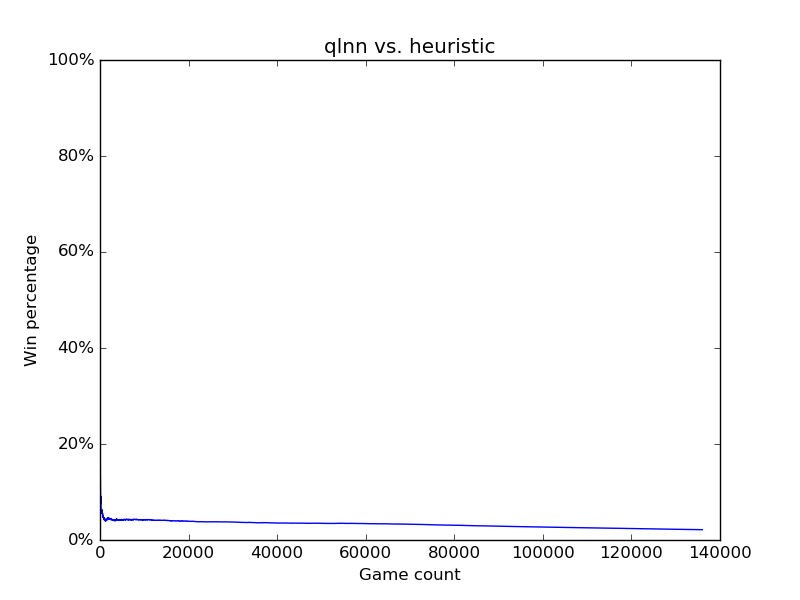
\includegraphics[width=0.50\textwidth]{4_133_160_187_140.png}
  \vspace*{-0.60cm}
  \caption{ANN(133, 160, 187, 140)}
  \label{fig:p1}
  \vspace*{-0.00cm}
\end{wrapfigure}

\begin{wrapfigure}{L}{0.5\textwidth}
  \vspace*{-0.00cm}
  \centering
  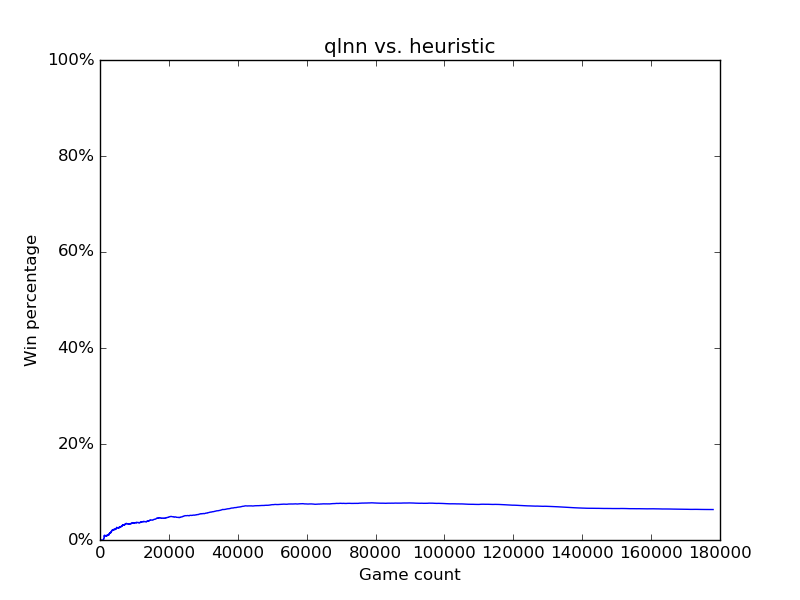
\includegraphics[width=0.50\textwidth]{4_133_200_200_140.png}
  \vspace*{-0.60cm}
  \caption{ANN(133, 200, 200, 140)}
  \label{fig:p2}
  \vspace*{-0.00cm}
\end{wrapfigure}

\begin{wrapfigure}{L}{0.5\textwidth}
  \vspace*{-0.00cm}
  \centering
  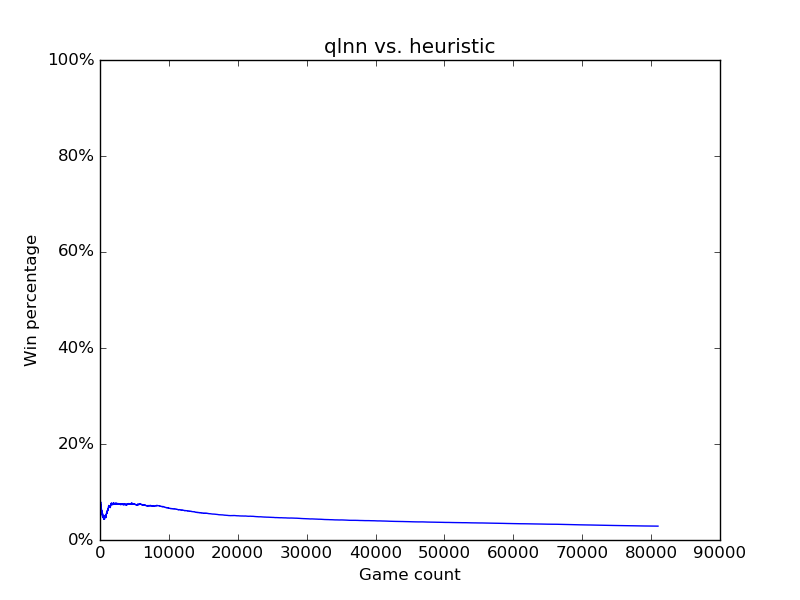
\includegraphics[width=0.50\textwidth]{4_133_345_140.png}
  \vspace*{-0.60cm}
  \caption{ANN(133, 345, 200, 140)}
  \label{fig:p3}
  \vspace*{-0.00cm}
\end{wrapfigure}

